\section{Terramechanics Revisited}
\label{s:Terramechanics_Revisited}
In section \ref{s:Terramechanics}, the established Bekker-Wong terramechanics theory for heavy class tracked vehicles in longitudinal motion was reviwed. This governs the gross traction effort $F$ and the relationship between terrain compaction resistance $R_c$ and sinkage $z$ from eq.'s \ref{eq:tractionForce}$-$\ref{eq:sinkage}.
\begin{linenomath*}
    \begin{equation*}
        F = (Ac + W\tan\Phi) \Big(1 - \frac{K}{il} \Big(1 - e^{\frac{il}{K}}\Big) \Big)
    \end{equation*}
\end{linenomath*}
\begin{linenomath*}
    \begin{equation*}
        R_c = b\bigg(\frac{k_c}{b} + k_\Phi\bigg)\frac{z^{n+1}}{n+1}
        %R_c = \frac{bl}{(n+1)(k_c/b + k_{\Phi})^{1/n}} \Big( \frac{W}{bl} \Big)^{n + 1/n}
    \end{equation*}
\end{linenomath*}
\begin{linenomath*}
    \begin{equation*}
        z = \bigg(\frac{W/A}{(k_c/b) + k_\Phi}\bigg)^{1/n}
        %p = \Big(\frac{k_c}{b} + k_{\Phi}\Big)z^n 
    \end{equation*}
\end{linenomath*}
Since the trajectories in this control mode are limited to longitudinal motion, an updated free body diagram is provided in Fig. \ref{fig:Free_Body_Diagram_Track_Longitudinal}. To capture a tractor's vulnerability to immobilization more accurately, the terramechanics theory used up this point must be augmented. 
\begin{figure}[b]
    \centering
    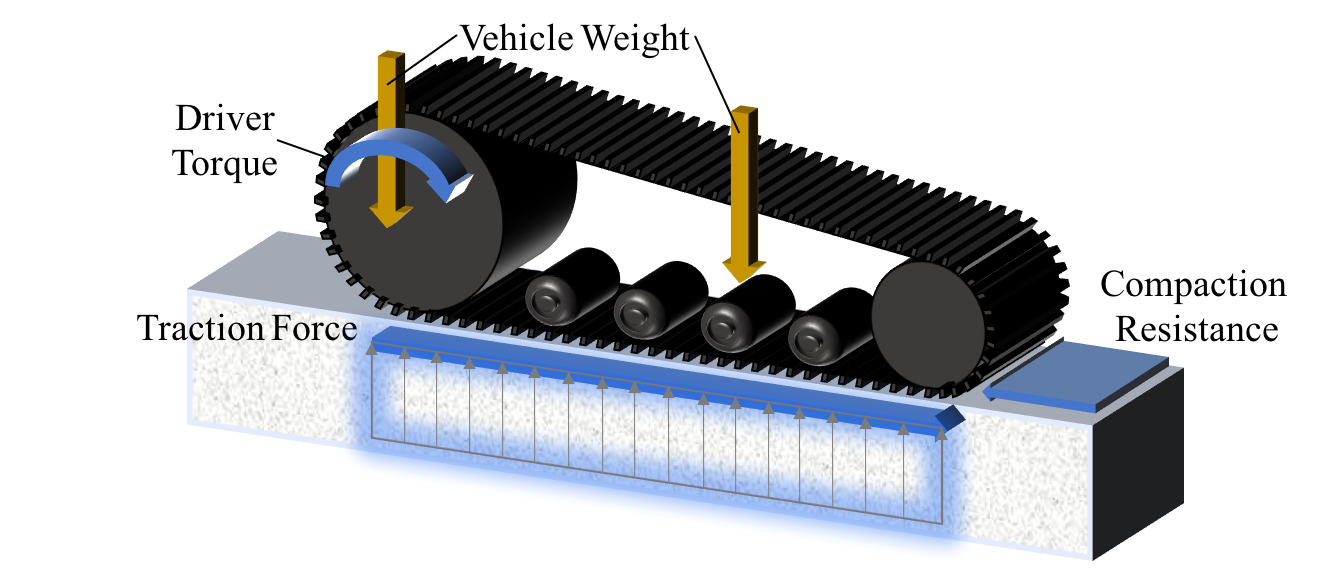
\includegraphics[width=5.5in]{Free_Body_Diagram_Track_Longitudinal}
    \caption{Track free body diagram for longitudinal motion}
    \label{fig:Free_Body_Diagram_Track_Longitudinal}
\end{figure}
Currently, Bekker-Wong theory has no inclusion of a slip-sinkage effect that is well established based on a set of terrain parameters. This slip-sinkage effect in real world environments is caused by excessive torque from the driver that overloads shear stresses on the terrain. This in turn causes terrain shear failure and excavation and the vehicle experiences increased sinkage and motion resistance. This phenomena was first investigated by Bekker and Reece \cite{Bekker1969,reece1965principles,reece1964problems}. However, no verifiable conclusions were reached. Recently, Lyasko has proposed an analytical formula for calculating dynamic sinkage for different slip values \cite{lyasko2010slip}. However, experimental data also show that the dynamic sinkage value can be calculated by
\begin{equation}\label{eq:slip_sinkage}
    z_D = z + iSz
\end{equation}
where $z_D$ is the dynamic sinkage from track slippage and $S$ is a slip-sinkage coefficient which is shown to be consistently close to $\frac{60\%}{33\%}$ \cite{lyasko2010slip}. This means that on average, slip values of 33\% result in an additional 60\% increase in sinkage from the static amount $z$. Equation \ref{eq:slip_sinkage} will be used to model the slip-sinkage effect to more accurately evaluate the effectiveness of the approach used for the traction control mode. Therefore, the equations for sinkage and compaction resistance from eq.'s \ref{eq:compactionResistance} and \ref{eq:sinkage} are now given by 
\begin{linenomath*}
    \begin{equation}
        R_c = b\bigg(\frac{k_c}{b} + k_\Phi\bigg)\frac{z_D^{n+1}}{n+1}
        %R_c = \frac{bl}{(n+1)(k_c/b + k_{\Phi})^{1/n}} \Big( \frac{W}{bl} \Big)^{n + 1/n}
    \end{equation}
\end{linenomath*}
\begin{linenomath*}
    \begin{equation}
        z_D = \bigg(\frac{W/A}{(k_c/b) + k_\Phi}\bigg)^{1/n} (1 + iS)
        %p = \Big(\frac{k_c}{b} + k_{\Phi}\Big)z^n 
    \end{equation}
\end{linenomath*}
The augmented terramechanics modeling discussed here results in a six dimensional terrain parameter space denoted by the vector $\mathbf{p}$
\begin{equation*}
    \mathbf{p} = \begin{bmatrix} c & \Phi & n & k_{eq} & K & S \end{bmatrix}^T
\end{equation*}